\documentclass[tikz,border=3.8mm]{standalone}
\usepackage[T1]{fontenc}
\usepackage{lmodern}
\usetikzlibrary{arrows.meta,calc}

\definecolor{concrete}{HTML}{EAF3FB}
\definecolor{abstract}{HTML}{FFF3C4}
\definecolor{ink}{HTML}{444444}

\begin{document}
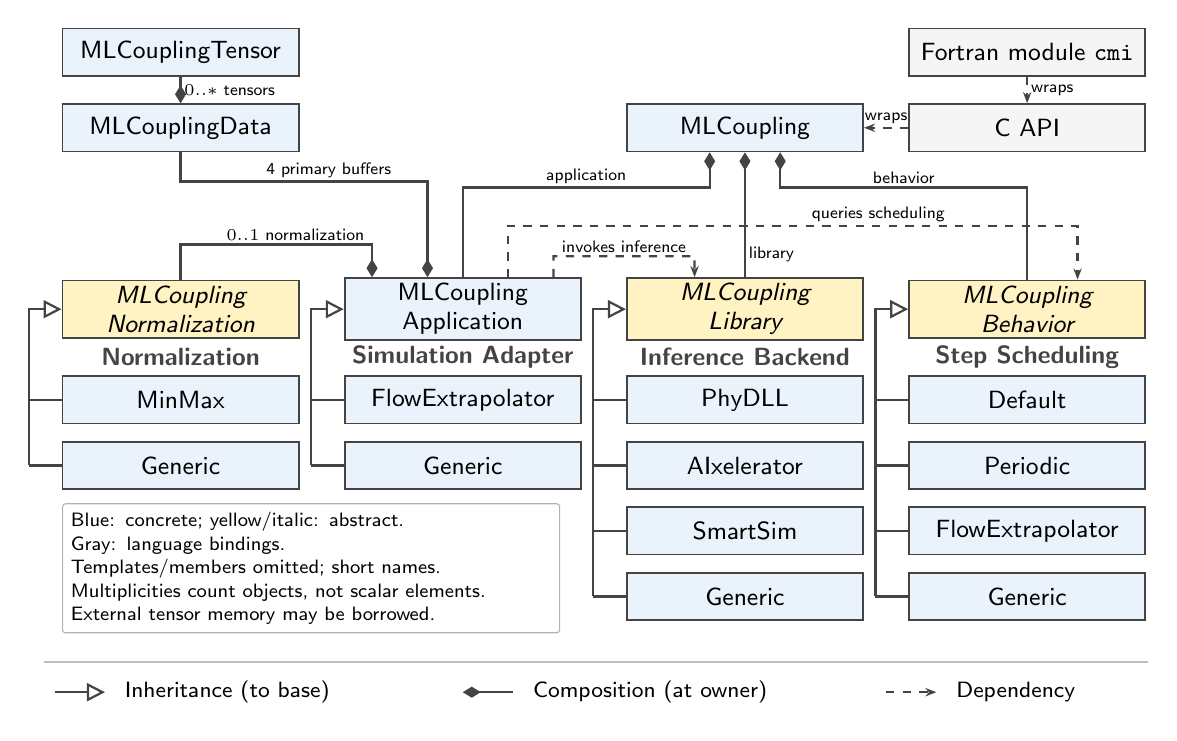
\begin{tikzpicture}[
  x=.64cm, y=.64cm,
  font=\sffamily\fontsize{9}{10.5}\selectfont,
  class/.style={draw=ink, line width=.65pt, fill=concrete,
    minimum width=3cm, minimum height=.6cm, align=center,
    inner sep=2pt},
  abstract/.style={class, fill=abstract, font=\sffamily\fontsize{9}{10.5}\selectfont\itshape},
  binding/.style={class, fill=gray!8},
  relation/.style={draw=ink, line width=.8pt},
  owns/.style={relation, {Diamond[length=6.5pt,width=4pt]}-},
  inherits/.style={relation, -{Triangle[open,length=6.5pt,width=6.5pt]}},
  dependency/.style={relation, dashed, -{Stealth[length=4pt,width=3pt]}},
  label/.style={font=\sffamily\fontsize{6}{7}\selectfont, inner sep=1pt},
  heading/.style={font=\sffamily\fontsize{9}{10.5}\selectfont\bfseries, text=ink}
]
% Fixed columns follow the sketch; connectors encode ownership, not data flow.
\node[class] (coupling) at (11.2,3.6) {MLCoupling};
\node[class] (data) at (0,3.6) {MLCouplingData};
\node[class] (tensor) at (0,5.1) {MLCouplingTensor};

\node[binding] (capi) at (16.8,3.6) {C API};
\node[binding] (fortran) at (16.8,5.1) {Fortran module \texttt{cmi}};
\draw[dependency] (fortran.south) -- node[label,right] {wraps} (capi.north);
\draw[dependency] (capi.west) -- node[label,above] {wraps}
  (coupling.east);

\node[heading] at (0,-.95) {Normalization};
\node[heading] at (5.6,-.95) {Simulation Adapter};
\node[heading] at (11.2,-.95) {Inference Backend};
\node[heading] at (16.8,-.95) {Step Scheduling};
\node[abstract] (normalization) at (0,0) {MLCoupling\\Normalization};
\node[class] (application) at (5.6,0) {MLCoupling\\Application};
\node[abstract] (library) at (11.2,0) {MLCoupling\\Library};
\node[abstract] (behavior) at (16.8,0) {MLCoupling\\Behavior};

\node[class] (minmax) at (0,-1.8) {MinMax};
\node[class] (normgeneric) at (0,-3.1) {Generic};
\node[class] (appflow) at (5.6,-1.8) {FlowExtrapolator};
\node[class] (appgeneric) at (5.6,-3.1) {Generic};
\node[class] (phydll) at (11.2,-1.8) {PhyDLL};
\node[class] (aix) at (11.2,-3.1) {AIxelerator};
\node[class] (smartsim) at (11.2,-4.4) {SmartSim};
\node[class] (libgeneric) at (11.2,-5.7) {Generic};
\node[class] (default) at (16.8,-1.8) {Default};
\node[class] (periodic) at (16.8,-3.1) {Periodic};
\node[class] (behflow) at (16.8,-4.4) {FlowExtrapolator};
\node[class] (behgeneric) at (16.8,-5.7) {Generic};

\draw[owns] ($(coupling.south)+(-.7,0)$) -- ++(0,-.7)
  -| node[label,pos=.25,above] {application} (application.north);
\draw[owns] (coupling.south) -- node[label,pos=.82,right] {library} (library.north);
\draw[owns] ($(coupling.south)+(.7,0)$) -- ++(0,-.7)
  -| node[label,pos=.25,above] {behavior} (behavior.north);
\draw[owns] ($(application.north)+(-1.8,0)$) -- ++(0,.65)
  -| node[label,pos=.2,above] {$0..1$ normalization} (normalization.north);
\draw[owns] ($(application.north)+(-.7,0)$) -- ++(0,1.9)
  -| node[label,pos=.2,above] {4 primary buffers} (data.south);
\draw[owns] (data.north) -- node[label,right] {$0..*$ tensors} (tensor.south);

% Application borrows these interfaces for ml_step(); it does not own them.
\draw[dependency] ($(application.north)+(1.8,0)$) -- (7.4,1.05)
  -| node[label,pos=.25,above] {invokes inference}
  ($(library.north)+(-1,0)$);
\draw[dependency] ($(application.north)+(.9,0)$) -- (6.5,1.65)
  -- node[label,pos=.65,above] {queries scheduling} (17.8,1.65)
  -- ($(behavior.north)+(1,0)$);

% Shared inheritance trunks have one hollow triangle pointing at each base.
\foreach \base/\last/\children in {
  normalization/normgeneric/{minmax,normgeneric},
  application/appgeneric/{appflow,appgeneric},
  library/libgeneric/{phydll,aix,smartsim,libgeneric},
  behavior/behgeneric/{default,periodic,behflow,behgeneric}} {
  \coordinate (trunk-\base) at ($(\base.west)+(-.65,0)$);
  \draw[inherits] (trunk-\base |- \last.west) -- (trunk-\base)
    -- (\base.west);
  \foreach \child in \children {
    \draw[relation] (\child.west) -- (trunk-\base |- \child.west);
  }
}

\node[draw=gray!60, rounded corners=1pt, inner sep=3pt,
  anchor=north west, align=left, text width=6.1cm,
  font=\sffamily\fontsize{7}{8.5}\selectfont]
  at (-2.35,-3.85) {
  Blue: concrete; yellow/italic: abstract.\\
  Gray: language bindings.\\
  Templates/members omitted; short names.\\
  Multiplicities count objects, not scalar elements.\\
  External tensor memory may be borrowed.
};
\draw[gray!50] (-2.7,-7) -- (19.2,-7);
\draw[inherits] (-2.5,-7.6) -- (-1.5,-7.6);
\node[anchor=west, font=\sffamily\fontsize{8}{9.5}\selectfont]
  at (-1.3,-7.6) {Inheritance (to base)};
\draw[owns] (5.6,-7.6) -- (6.6,-7.6);
\node[anchor=west, font=\sffamily\fontsize{8}{9.5}\selectfont]
  at (6.8,-7.6) {Composition (at owner)};
\draw[dependency] (14,-7.6) -- (15,-7.6);
\node[anchor=west, font=\sffamily\fontsize{8}{9.5}\selectfont]
  at (15.2,-7.6) {Dependency};
\end{tikzpicture}
\end{document}
